\secspace
\section{Evaluation of IMPRESS}
\label{sec:issues}

Here, we first identify a few flaws in IMPRESS's experiment setup 
and then evaluate purification performance 
in several realistic mimicry scenarios. 

\para{Setup. } We follow the purification setup from the original IMPRESS paper and the source
code provided by the authors. We use default 
Glaze setup (perturbation budget = $0.07$) as described in the paper. 
We follow style mimicry setup in prior 
work~\cite{shan2023glaze}. Given a set of artworks, we mimic its style by
fine-tuning stable diffusion model (version 1.5) using DreamBooth 
for 600 to 1000 steps depending on the finetuning sample size for the artist.

\begin{figure*}
  \centering
  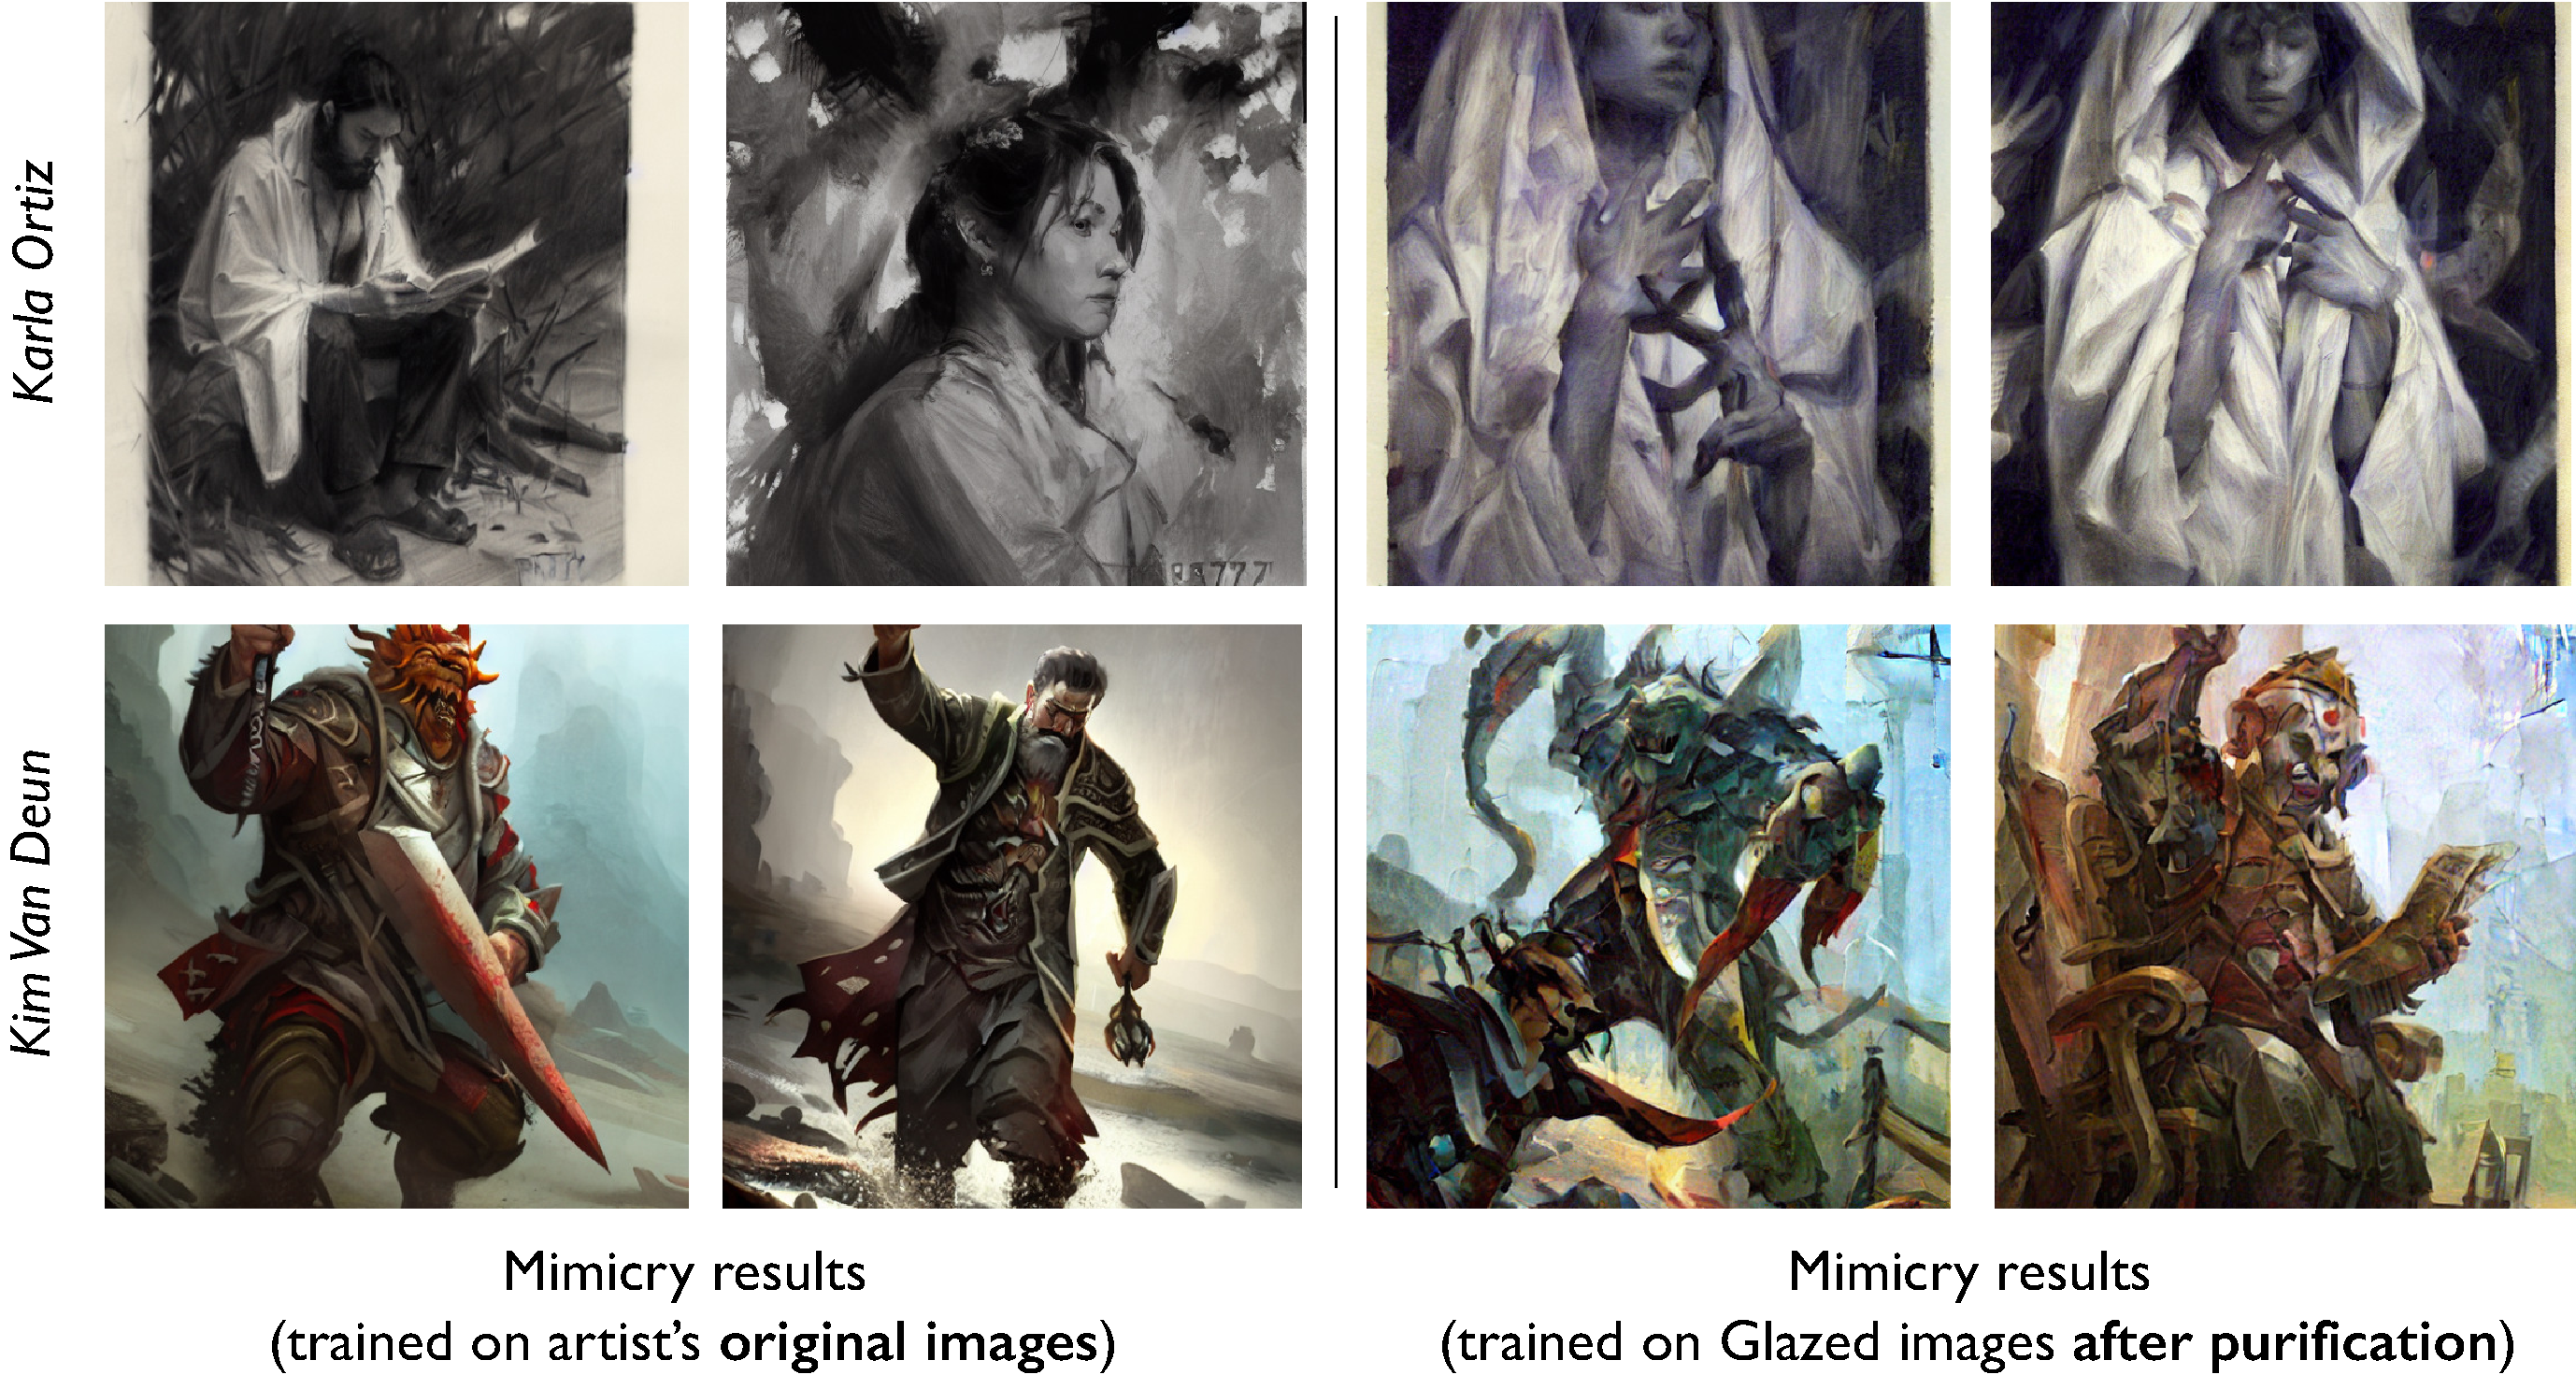
\includegraphics[width=0.99\linewidth]{nonhistorical.pdf}
  \vspace{-0.1in}
  \caption{Mimicry results on non-historical artists (Karla Ortiz and Kim van Deun). Left shows the images generated from a model trained on original images; right shows the images generated from a model trained on images that are first Glazed and then purified by IMPRESS. }
  \label{fig:non-historical}
  \vspace{-0.in}
\end{figure*}

\begin{figure*}
  \centering
  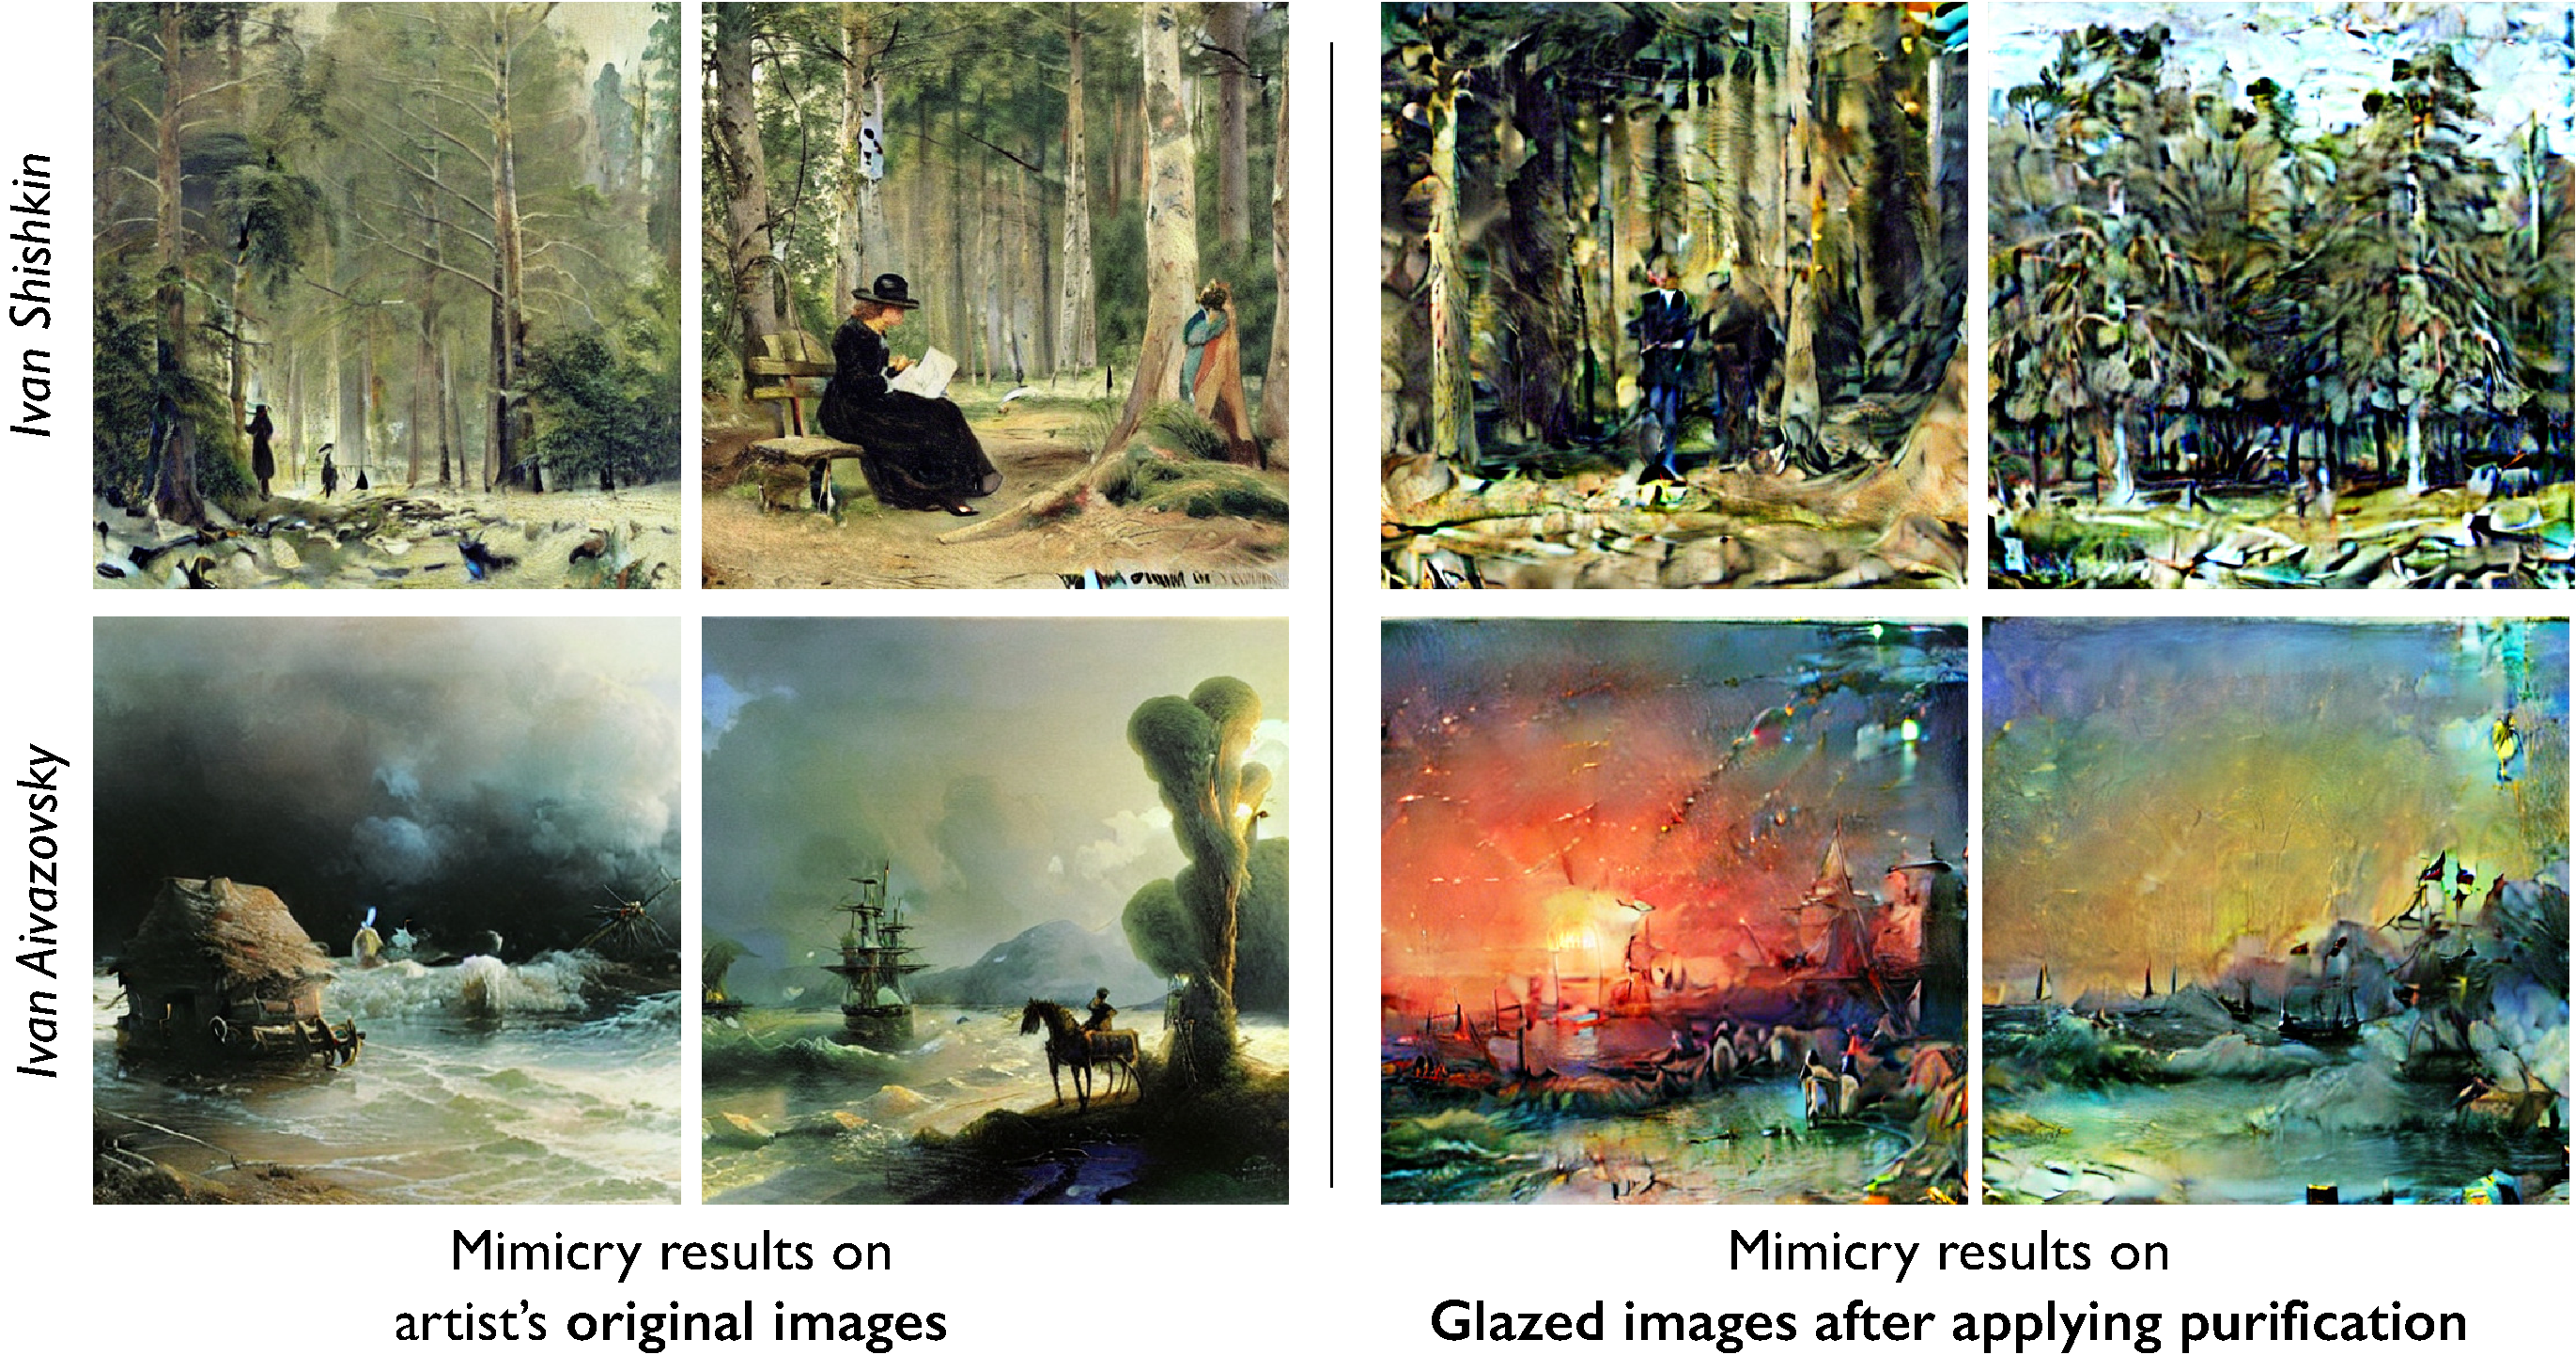
\includegraphics[width=0.99\linewidth]{smooth.pdf}
  \vspace{-0.1in}
  \caption{Mimicry results on smooth surface art styles (Ivan Shishkin and Ivan Aivazovsky). Left shows the images generated from a model trained on original images; right shows the images generated from a model trained on images that are first Glazed and then purified by IMPRESS. }
   \label{fig:smooth}
  \vspace{-0.in}
\end{figure*}

\begin{figure*}
  \centering
  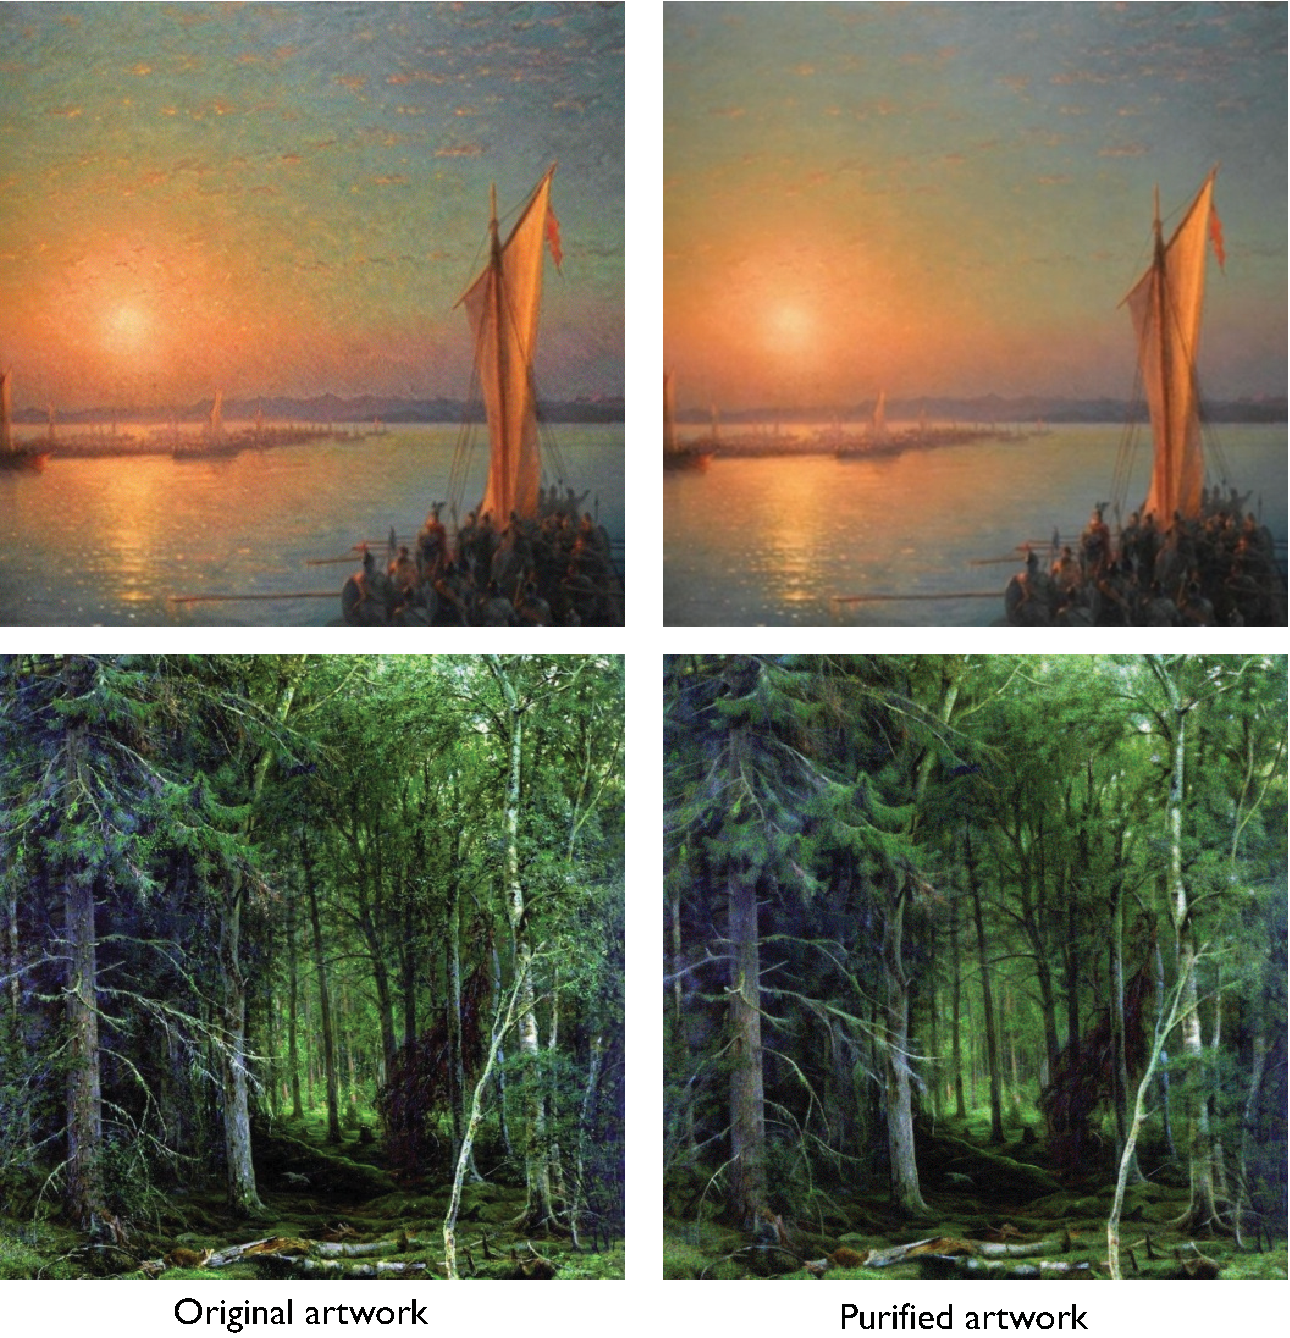
\includegraphics[width=0.95\linewidth]{clean-degrade.pdf}
  \vspace{-0.1in}
  \caption{Original artwork and corresponding purified artwork. }
  \label{fig:clean}
  \vspace{-0.in}
\end{figure*}

\subsection{Generalizability to Realistic Scenarios}

In the original IMPRESS paper, the authors focus the evaluation on protecting the
art styles of famous historical artists (Monet, Van Gogh) -- whose style are already learned
by pretrained diffusion models prior to style mimicry. In the real-world, it is current artists
who are most concerned about AI mimicking their art style. Glaze is designed
to protect those artists, and they are not as heavily pretrained into the
base model as Monet or Van Gogh. 

We evaluate IMPRESS on non-historical artists and show that purification
has limited effectiveness at removing Glaze protection. 
Even for historical artists, we find the purification works poorly for 
certain art styles. Lastly, we find purification also degrades clean image quality where
it removes texture from art pieces. 

\para{Performance on non-historical artists. } We use artwork from Karla 
Ortiz and Kim Van Deun to simulate the mimicry attack on current artists. Karla is a fine-art artist 
with a similar style as some historical artists tested in the IMPRESS paper. 
Figure~\ref{fig:non-historical}
shows the mimicry results when model trained on artist's original art pieces (left)
or when model trained on art pieces that are first Glazed
and then purified by IMPRESS (right). We can observe significant amount of 
artifacts on mimicry results when the model is trained on purified Glazed images. 

\para{Poor performance on certain art styles. } IMPRESS works by adding artifacts
on Glazed images to recover the latent representation of original artwork. 
We found purification has more challenges recovering smooth surface 
art styles (realism art, symbolism, romanticism, etc) even for historical
artists already trained into the base model. 
We choose two historical artists: Ivan Aivazovsky (romanticism style) and Ivan Shishkin (realism style). 

Figure~\ref{fig:smooth} shows the mimicry results. We see IMPRESS 
introduces signficiant amount of artifacts to the mimicked images. 
The weaker performance is likely because purifying  the 
original smoother surface art requires the optimization to 
be very percise -- find the exact smooth surface. 

\para{Degrading image quality. } We found the purification process degrades 
clean image quality. Figure~\ref{fig:clean} shows original artwork 
and its corresponding purified artwork. The purified artwork is much more
blurry as purification removes textures from the images. 

\subsection{CLIP-based metrics are Inaccurate}

``CLIP genre accuracy'' quantifies if mimicked art is classified into the same art genre as the original 
art pieces according to a CLIP model. It has been used in prior work to evaluate mimicry 
success. However, in our own tests dating back to late September 2023, we
found CLIP genre accuracy is a poor indicator of end-to-end mimicry success.  
CLIP accuracy is especially poor when evaluating attacks against Glaze. The 
reason is that attacks (such as 
IMPRESS purification), as they seek to remove Glaze effect from art, often have signficant impact 
on the base image quaility of the artwork. 
The degradation in image quality is not captured by CLIP accuracy, \eg a very
low quality cubism painting is still classified as ``cubism'' with high
probability. But the result are not successful 
mimicry due to the low quaility of the mimicked images. 
Because of these poor properties as an accuracy indicator, we stopped using
CLIP distance as a success metric starting with the Glaze v1.1 update
(October 2023). 
